%!TEX root = ../dissertation.tex

\chapter{Background}
\label{chapter:Background}

This chapter provides fundamentals of theoretical knowledge required to understand the work for the previously stated problem. Firstly, we will discuss about object detection and feature extraction with presentation of the state of the art solution used (section \ref{Object_detection}). Secondly, we will describe the visual servoing control theory and solutions (section \ref{Visual_Servoing}). Thirdly, we will explain what is a manipulator in terms of robotics and what is kinematics of robotic manipulators (section \ref{Robotic_manipulator}).

\section{Object Detection and Features Extractions}
\label{Object_detection}

Object detection is the fist step performed by the presented controller. This detection is used to classify and track the object in real-time when the manipulator is moving (since the camera is fixed to the end effector) but also if the object is moved since the controller is used in a dynamic environment. Feature extraction is the second step performed by the controller and is used to compute the visual servoing control law.

\subsection{Objection detection}

Objection detection is a classical problem in computer vision, and it can be stated as recognize what the objects are inside a given image and also where they are in the image. To achieve this task, this work use a state of the art object detection algorithm called \gls{YOLO} \cite{DBLP:journals/corr/RedmonDGF15}.
\gls{YOLO} is a convolutional neural network that was introduced in 2015 and recently improved its accuracy and speed on object detection with YOLOv2 \cite{DBLP:journals/corr/RedmonF16}. It is an object detection system targeted for real-time processing. 

\subsubsection{Functioning}

The first step is given an image, YOLO starts by splitting that image into an n\*n grid cells (figure : \ref{pict:yolo_grid}). In this grid, each of the cells (in red, in figure \ref{pict:yolo_grid}) is responsible for predicting n bounding box associate with a confidence score. 

\newpage

\begin{figure} [!ht]
    \centering
    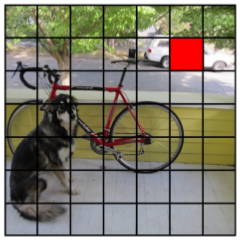
\includegraphics[width=0.4\linewidth]{images/yolo_grid.png}
    \caption{Image splitted into a n*n grid, from YOLO website}
    \label{pict:yolo_grid}
\end{figure}

Each individual bounding box confidence score tells you how certain YOLO is that the predicted bounding box actually contains an object and also how well the bounding box feats the object.

\begin{figure} [!ht]
    \centering
    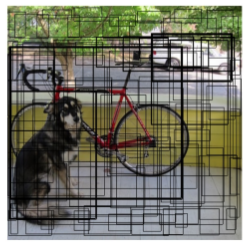
\includegraphics[width=0.4\linewidth]{images/yolo_confidence.png}
    \caption{Resulting prediction from all the grid cells (the thickness of the bounding box increase with the confidence, from YOLO website}
    \label{pict:yolo_confidence}
\end{figure}

In figure \ref{pict:yolo_confidence}, the prediction from all the cells regrouped together is visualized. This prediction take the aspect of many bounding box ranked by their confidence score. This way you know more or less where objects are in the image but you don't know what is the object.

The second step is for each cells (figure: \ref{pict:yolo_grid}) YOLO predicts a  class conditional probabilities. It only predicts one set of class probabilities per cell, regardless the number of bounding box associated with that cell. Note that since its using conditional probabilities, if a cell predict an object for example a bike it doesn't mean that inside of this cell there is this bike, it only means that if there is an object inside this bounding box then this object is a bike (figure \ref{pict:yolo_proba}).

\newpage

\begin{figure} [!ht]
    \centering
    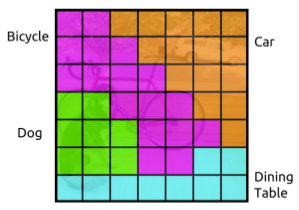
\includegraphics[width=0.4\linewidth]{images/yolo_proba.png}
    \caption{ Class conditional probability map from YOLO website}
    \label{pict:yolo_proba}
\end{figure}

The third step is to combine both previous step (confidence score for the bounding box and class conditional probabilities) into one final score. This final score evaluates the confidence that each bounding box contains a specific object (figure \ref{pict:yolo_final}).

\begin{figure} [!ht]
    \centering
    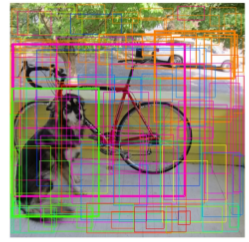
\includegraphics[width=0.4\linewidth]{images/yolo_final.png}
    \caption{Bounding box and class conditional probabilities, from YOLO website}
    \label{pict:yolo_final}
\end{figure}

In figure \ref{pict:yolo_final}, their are still a lot of bounding box, the only remained step is to filter this bounding box with a final score that has to be higher than a specific threshold. Also, duplicated bounding boxes are removed using a non-maximum suppression. The final result is visible on figure \ref{pict:yolo_final_filter}.

\begin{figure} [!ht]
    \centering
    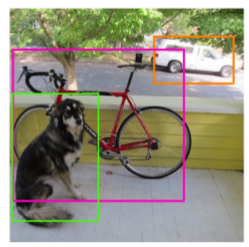
\includegraphics[width=0.3\linewidth]{images/yolo_final_filter.png}
    \caption{Final result after filtering, output from YOLO, from YOLO website}
    \label{pict:yolo_final_filter}
\end{figure}

\newpage

To summarize, each of the bounding boxes are composed by 5 predictions:
\begin{enumerate}
    \item x,y coordinates: offsets between the center of the bounding box relatives to the bounds of the cell.
    \item w,h: width and height of the bounding box
    \item confidence score, how YOLO is certain that this bounding box contains this object
\end{enumerate}

YOLO is a state of the art solution because it is a real time object detection system. What is the secret ? The output predictions are all computed at the same time looking only once the image (You Look Only Once). Since it predicts all of these detection simultaneously YOLO also implicitly incorporates global context in the detection process so it can learn things about which objects tend to occur together, the relative size and location of objects and other assorted things.

\subsubsection{Training}

YOLO is pre-trained on a ImageNet that is currently the biggest dataset for Computer Vision tasks (millions of images, more than a thousands class in different scenes). When pre-train, it learns to convert the millions images into a feature map (convolution weights). So when YOLO is actually trained with your own data set it adapts this convolutional weights to detect your own object class in the training set of images. Pre-train allows to have very good performance with a small training set. 

For the data augmentation, YOLO randomly scales and translates of up to 20\% of the original image size and also randomly adjusts the exposure and saturation of the image by up to a
factor of 1.5 and hue by up to a factor 0.1 in the HSV color space.

Overall the training of this network is straightforward and corresponds to a lot a of standards in the Computer Vision community: YOLO pre-train on ImageNet, uses stochastic gradient descent and uses data augmentation.

\begin{figure} [!ht]
    \centering
    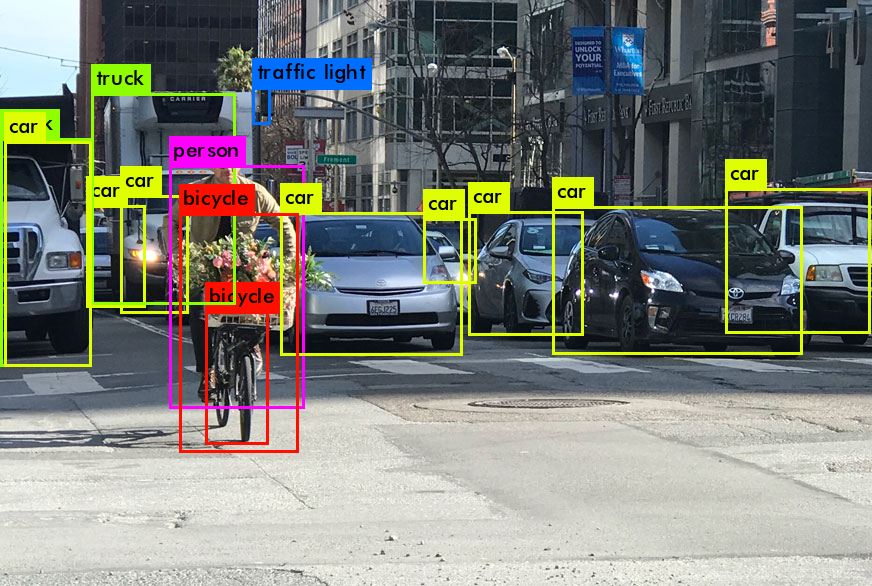
\includegraphics[width=0.65\linewidth]{images/yolo_example.png}
    \caption{YOLO at work, street road example}
    \label{pict:yolo_example}
\end{figure}


\newpage

\subsection{Feature Extraction}

Feature extraction is the second step performed by the presented controller.

\subsubsection{Image feature}

Image feature is a simple image pattern, based on which what we see in the image can be described. The main role of features in computer visions is to transform visual information into the vector space. On the vector space we will be able to apply mathematical operations on this features.
This features can be for example points, lines or ellipses.
The selected feature as what his called a feature parameter, it is any numerical quantity associated to the selected feature in the image plane. This can be coordinates of a point, angular coefficient and offset of a line, center and radius of a circle, generalized moments of an object in the image.

\subsubsection{Image Formation}

In this section, the image acquisition process will be described. To this purpose we will use the perspective camera model. It is the model the most commonly used in computer vision, it reproduces with the behaviour of real cameras with the most accuracy \cite{Szeliski:2010:CVA:1941882}.

\begin{figure} [!ht]
    \centering
    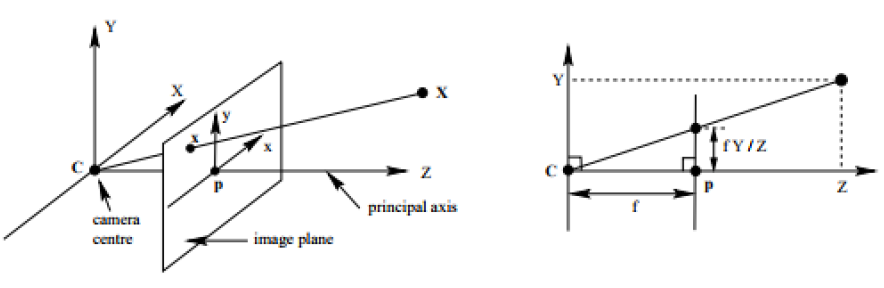
\includegraphics[width=0.65\linewidth]{images/model.png}
    \caption{Ideal pinhole camera model}
    \label{pict:pinhole_camera_model}
\end{figure}

Given a 3D scene in the world, a camera projects one or more 3-D point(s) onto the 2D image plane. The main feature of the perspective projection is the conservation of straight lines, after the transformation. The image formation can be described with a model called the pinhole camera model \cite{Hartley2004} (Figure: \ref{pict:pinhole_camera_model}).

Figure \ref{pict:pinhole_camera_model} shows the ideal representation of the pinhole camera model, considering a central projection of points in space, onto an image plan defined by $Z = f$ where $f$ is the focal length. The optical center $C$, located at the origin of this 3D coordinate system, represents the point in which all the 3D projection intersect. This principal axis is defined as the line perpendicular to the image plane, passing through the optical center. The principal axis intersects the image plane in the principal point $p$ \cite{Hartley2004}.

A point $X = (X,Y,Z)^T$ defined in the coordinate system of the camera, is mapped on the image, dividing the coordinates X and Y by the point depth Z, and multiplying by the focal length f as described in

\begin{equation}
    X = (X,Y,Z)^T = (f \frac{X}{Z},f \frac{Y}{Z})^T
    \label{eq_image_1}
\end{equation}
\newpage

Using homogeneous coordinates (\ref{eq_image_1}) can be written as:
\begin{equation}
   x = PX
\end{equation}
With $ x = (f \frac{X}{Z},f \frac{Y}{Z})^T $ and $ X = (X, Y, Z, 1)^T$ and the camera matrix P is composed by the matrix $K$ of intrinsic parameters and the extrinsic parameters matrix composed by the rotation matrix $R$ and the translation matrix $t$.
\begin{equation}
   P = K \big[ R|t \big]
\end{equation}
The matrix K of intrinsic parameters, also called calibration matrix can be represent as:
\[
K 
=
\begin{bmatrix}
    f_{x} & s & c_{x} \\
    0 & f_{y} & c_{y}\\
    0 & 0 & 1
\end{bmatrix}
\]
where $f_{x}$ and $f_{y}$ are independent focal length for the camera sensor x and y dimensions. $c_{x}$ and $c_{y}$ denotes the optical frame center expressed in pixel coordinates.

$X$ will be expressed in the camera coordinate frame but the points in 3D space are expressed in the world coordinate frame. The extrinsic parameters matrix (E)  represent the relation between this two spaces. It represents the external position and orientation of the camera in the 3D world and relates the camera frame to the world frame:
\[
E
=
\begin{bmatrix}
    R_{[3x3]} & t \\
    0_{[1x3]} & 1
\end{bmatrix}
\]
an homogeneous matrix composed by a rotation matrix (R) and a translation vector (t).\\

To resume, in this section we have been looking into general knowledge about image features and image formation. Object detection and feature extraction are the first step in the algorithm that will be describe in the next chapter.
\newpage
\section{Visual Servoing}
\label{Visual_Servoing}

\gls{VS} relies on techniques from areas like image processing, computer vision, and
control theory. Here, we present a definition of VS, Image-Based Visual Servoing (IBVS), \gls{PBVS}, and Hybrid method. Different ways of classifying these techniques are possible. Several classifications are extensively discussed in \cite{Staniak:2010:SVS:1831760.1831963}.
VS is the use of the vision to extract features and to process images to control robot pose. The introduction to visual feedback makes the system less sensitive to errors that could be generated by inadequate calibration, noise in the system or changes in the environment. Contrarily to open-loop approaches, like "looking" then "moving" methods, the use of visual information acquired in real time, makes the control scheme more robust and adaptive. VS, using visual-feedback control loop, increases the overall accuracy of the systems and appears as an attractive technique to achieve manipulation tasks.

When doing visual servoing two camera configurations are defined: EYE-IN-HAND and EYE-TO-HAND (figure:\ref{pict:eye_in_hand})
\begin{figure} [h]
    \centering
    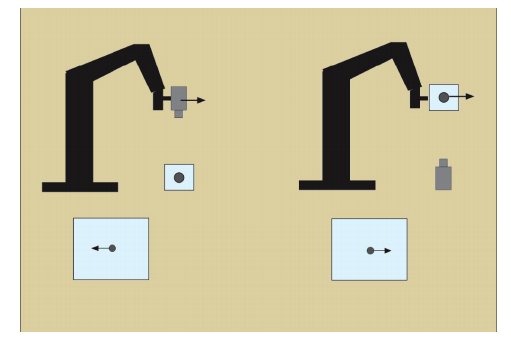
\includegraphics[width=0.65\linewidth]{images/eye_un_hand.png}
    \caption{EYE-IN-HAND (on the left) and EYE-TO-HAND (on the right) configuration}
    \label{pict:eye_in_hand}
\end{figure}\\
Based on \cite{<inria-00350283>}, we will describe the various basic approaches in \gls{VS}. 

\subsection{Image Base Visual Servoing}
\label{chap:ibvs}

IBVS uses measurements in the image m(t) (pixel coordinates, lines, moments
of region,...) converted to features using camera intrinsic parameters
p. The error signal is measured directly from the image. The control law is
based on the computed error between the set of current visual features and the set of 
desired features given by $s^*$. The interaction matrix relates a 2D point projected in
the image from a 3D point in the camera frame, by the depth of the point in
the camera frame
The error is defined as:
\begin{equation}
\label{first_ibvs}
e(t)=s(m(t),p) - s^*
\end{equation}
with m(t), the computation from the image measurements, e.g. image coordinates of interest point, area, center of gravity.
p, other parameters like camera intrinsic parameters, 3D models of objects or the pose between camera and environment.
The time variation of $s$, $\Dot{s}$ and the camera spacial velocity, $v_{c}$ has been related by Chaumette in \cite{<inria-00350283>} like:

\begin{equation}
    \Dot{s} = L_{s}v_{c}
    \label{equation_1_ibvs}
\end{equation}
with $v_{c} = (v_{c}, w_{c})$, describing linear velocities and angular velocities relative to the origin of the camera frame.
$L_{s}$, is  called the interaction matrix (k, number of visual features * N, number of robot DoF).

The time variation of the error is equal to the time variation of the current features:
\[
\Dot{e} = \Dot{s}
\]
From \ref{equation_1_ibvs}, we can relate the time variation of the error with the precedent relation:
\begin{equation}
     \Dot{e} = L_{s}v_{c}
     \label{equation_2_ibvs}
\end{equation}
The goal is to reduce the error, to make the error converge to a lower value, to achieve this purpose an exponential decay was introduced \cite{<inria-00350283>} :
\begin{equation}
     \Dot{e} = - \lambda e
\end{equation}
From \ref{equation_2_ibvs} and since the control is done on the camera velocities the control law becomes:
\begin{equation}
\label{eq_control_law}
    v_{c}= - \lambda L_{s}^+ e
\end{equation}
with $L_{s}^+$ the Moore-Penrose pseudo inverse matrix, that is defined as:
\[
L_{s}^+ = (L_{s}^T L_{s})^{-1} L_{s}^T
\]
when $(L_{s}^T L_{s}$ is of full rank. Both $L_{s}^T$ and $L_{s}$ are hard to be exactly computed in real \gls{VS} systems. They have to be estimated as $\hat{L_{s}}$ in the control law. 

From a 3D point coordinates (X,Y,Z) and related to the image formation subsection, the point coordinates are defined in the image plan as:
\begin{equation}
    \begin{aligned}
    x = X / Z \\
    y = Y / Z
    \end{aligned}
\end{equation}
From this point coordinates, the current features and desired features are constructed: 
\begin{equation}
    \begin{aligned}
     s = (x, y)\\
     s^* = (x, y) 
    \end{aligned}
\end{equation}
Now, the time variation of the previous point coordinates can be written as:
\begin{equation}
\label{eq1_interaction}
    \begin{aligned}
    \Dot{x} = (\Dot{X} - x\Dot{Z})/Z \\
    \Dot{y} = (\Dot{Y} - y\Dot{Z})/Z
    \end{aligned}
\end{equation}
Relating the velocity of the 3D point with the camera spatial velocity is given by:
 \begin{equation}
 \label{eq32_interaction}
    \Dot{X} = - v_c - w_c * X
 \end{equation}
Becomes:
\begin{equation}
\label{eq2_interaction}
    \begin{aligned}
    \Dot{X} = - v_x - w_y * Z + w_z*Y \\
    \Dot{Y} = - v_x - w_y * Z + w_z*Y \\
    \Dot{Z} = - v_x - w_y * Z + w_z*Y
\end{aligned}
\end{equation}
Now using (\ref{eq2_interaction}) inside (\ref{eq1_interaction}):
\begin{equation}
\label{eq3_interaction}
    \begin{aligned}
    \Dot{x} = - \frac{v_x}{Z} -(1+x^2)w_y + w_z y + \frac{x}{Z} v_z + x y w_x \\
    \Dot{y} =- \frac{v_y}{Z} + (1+x^2)w_x + w_z x + \frac{x}{Z} v_z - x y w_y \\
\end{aligned}
\end{equation}
\ref{eq3_interaction} can be written as:
\begin{equation}
    \Dot{x} = L_x v_c
\end{equation}
Finally, the interaction matrix related to the 3D point is:
\[
\begin{bmatrix}
    - \frac{1}{Z} & 0 & \frac{x}{Z} & x y & -(1+x^2) & y \\
    0 & - \frac{1}{Z} & \frac{y}{Z} & 1+y^2 & - x y & x 
\end{bmatrix}
\]
If more than one point is used, the global interaction matrix will be stacking intermediate interaction matrix. For example if 3 points are used $x = (x_1, x_2, x_3)$:
\[
L_x
=
\begin{bmatrix}
    L_{x1} \\
    L_{x2} \\
    L_{x3} 
\end{bmatrix}
\]

This matrix has to be estimated when used in control law and the quantity of points chosen has to be enough to avoid singular configurations and local minima.
They are several methods to estimate the interaction matrix in IBVS \cite{<inria-00350283>}. 

The most straight forward method is to estimate the current depth Z of each point, at each iteration of the control scheme:
\[
\Hat{L_s^+} = L_s^+ 
\]
According to \cite{<inria-00350283>}, this method gives a good local behavior but the global behavior is unsatisfactory. It means that the convergence will not be as good as expected.

Another approach is to set only the desired depth $Z^*$ of each point for the desired pose:
\[
\Hat{L_s^+} = L_{s^*}^+ 
\]
According to \cite{<inria-00350283>}, this method gives a good local behavior but introduce unexpected translational motion. 

A minimization approach as lately been proposed \cite{1308092} leading to chose:
\[
\Hat{L_s^+} = \frac{1}{2}(L_{s^*}^+ + L_s^+)
\]
This method gives a better trajectory with less oscillations. \\

Problems from using a \gls{IBVS} are referred in literature, like problems of singularities in the interaction matrix, or the reach of local minima can lead to problem in the control. It is also known as a highly coupled process. A correct estimation of the interaction matrix in IBVS is important to provide stability to the control system and avoid perturbations. 

\subsection{Pose Based Visual Servoing}
\label{chap:pbvs}

\gls{PBVS} uses 3D features instead of 2D, as in IBVS, required to estimate the
pose of the targeted object. Features are extracted from the image and used to
determine the pose of the target with respect to the camera, in the Cartesian space \cite{<book-coork>}. Various methods of 3D pose computation of an object exist in the literature from triangulation methods, to model based estimation. The classical computer vision problem is called the 3D localization problem \cite{LOWE1987355}. Once the 3D reconstruction of the object is established, the error is then computed in the task space and used in the control law.
All the previous step of the control law computation from (eq: \ref{first_ibvs}) to (eq: \ref{eq_control_law}) presented in the previous section are still valid. However, the interaction matrix will not be the same. \\

Four coordinate frames are considered: the current camera frame $C$, the world base frame $W$, an object frame $O$, as reference of frame of the object and  a desired camera frame $C^*$. The orientation of $C$ relative to $C^*$ is given by a rotation matrix $R_{[3x3]}$. The corresponding angle parametrisation $\theta$ and the translation vector t, defines the feature s.
The computation of the interaction matrix will then depend on how t is defined:

If t is defined as a function of $O$, $t^C_O$, $\theta = 0$ for the desired feature $s^*$  and the error is computed between  $t^C_O$ and $t^{C^*}_O$
\[
L_e
=
\begin{bmatrix}
    -I_3 & t \\
    0 & L_\theta
\end{bmatrix}
\]
with $I_3$ the identity matrix.
If t is defined as a function of $C$, $t^{C^*}_O$, $m^* = 0$ and $e=s$, the interaction matrix will be:
\[
L_e
=
\begin{bmatrix}
   R^{C^*}_C & 0 \\
    0 & L_\theta
\end{bmatrix}
\] \\

Usually the trajectory is better followed in 3D space than in image space due to the definition in Cartesian space. However, points can leave the image space due to the fact that the control is not directly done in the image. In PBVS a correct estimation of the pose is crucial, because of the error regulation. So the 3D reconstruction depends directly on the calibration of the vision system.

\begin{figure} [!ht]
    \centering
    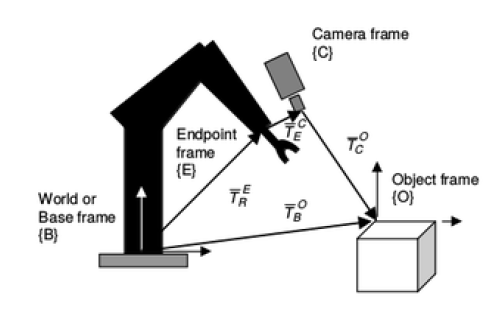
\includegraphics[width=0.5\linewidth]{images/coordinates_frame_pbvs.png}
    \caption{PBVS, coordinate frames overview}
    \label{pict:pbvs}
\end{figure}

\subsection{Hybrid}
\label{hybrid}

In the two previous sections, the two main methods for \gls{VS}, where presented. A combination of these methods is also possible, it is called Hybrid visual servoing. The basic idea behind hybrid visual servoing is to decouple the Z axis motions (including
both the translational and the rotational components) from the other DoF. In this section, one method of hybrid visual servoing will be presented but it is not the only possibilities, more methods are present in the literature. 
The 2-1/2D visual servoing is an hybrid method. The main idea is to control the camera motion with both IBVS and PBVS. IBVS will be use to control the translational motion and PBVS to control the rotational motion. In \cite{<inria-01350283>}, starting from the hypothesis that a control for angular velocity $w_c$ is available, in PBVS method can be defined as:

\begin{equation}
    w_c = - \lambda \theta
\end{equation}
The goal is to control the several translational DoF by partitioning the interaction matrix into two matrices: $L_v$, matrix of linear velocities, and $L_w$, matrix of angular velocities, obtaining:
\begin{equation}
    L_e
=
\begin{bmatrix}
   L_v & L_w \\
    0 & L_\theta
\end{bmatrix}
\end{equation}
Now, the time variation of the feature can be describe as:
\begin{equation}
    \Dot{s}
=
\begin{bmatrix}
   L_v & L_w 
\end{bmatrix}
\begin{bmatrix}
   v_c \\ 
   w_c
\end{bmatrix}
\end{equation}
The desired translation control input is solved for an error with an exponential decay:
\begin{equation}
    \Dot{e_t} = -\lambda e_t
\end{equation}
At the end, the following control law is obtained to express the translational motion input:
\begin{equation}
    v_c = - L_v^+(\lambda e_t + L_w w_c)
\end{equation}
 with $\lambda e_t + L_w w_c$, the new error expression. \\

To resume, in this method, the translational velocities are computed from an IBVS control law and the rotation velocities can be added later using a 3D pose estimation algorithm and compute using PBVS visual servoing. 


\section{Robotic manipulators and kinematics}
\label{Robotic_manipulator}

Robotic servo manipulators are kinematic chains.They are composed of links, and this links are connected by joints (figure: \ref{pict:chain}). The fixed part of the chain is called the base and the ending part is called the end effector. It is where usually the tool performing the task (effector) is fixed, for example a gripper. In robotic manipulators joints are the movable elements, which enable relative movement between the neighboring links. \\

\begin{figure} [!ht]
    \centering
    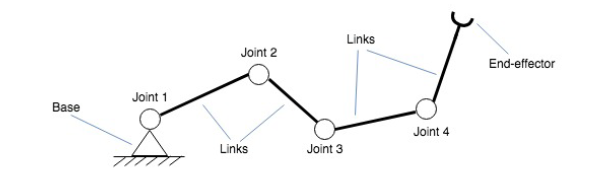
\includegraphics[width=0.65\linewidth]{images/chain.png}
    \caption{Kinematic chain of manipulator}
    \label{pict:chain}
\end{figure}

To describe the position and orientation of the robotic manipulator in space, frames are attached to the links and to the end effector (figure: \ref{pict:frames}). Each frame is expressed with respect to a reference frame called base frame. Description of the frame is given by position vector (position description) relative to some other reference frame and rotation matrix (orientation description).

\begin{figure} [!ht]
    \centering
    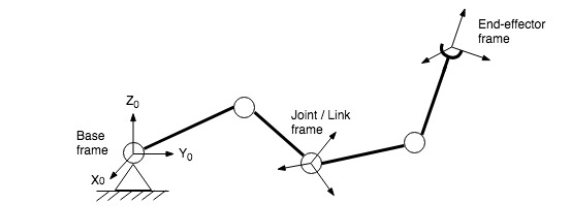
\includegraphics[width=0.65\linewidth]{images/frames.png}
    \caption{Frames attached on the manipulator joints}
    \label{pict:frames}
\end{figure}
This transformation is stored in an homogeneous matrix:
\[
T
=
\begin{bmatrix}
    R_{[3x3]} & t \\
    0_{[1x3]} & 1
\end{bmatrix}
\]

To compute transformation between base frame and last link, kinematic equations are use. For example, the transformation from frame {i} to frame {0} (base frame) can be written:

\begin{equation}
    T_i^0=T_1^0 T_2^1 ... T_i^{i-1}
\end{equation}
The transformation is a function of all joint variables and it computes Cartesian position and orientation of the last link frame.

\subsection{Forward kinematics}
\label{chap:forwardkinematics}


Knowing simple geometrical manipulator’s frames positions, in respect to other adjacent frames, it is possible to compute coordinates of the end effector, from the given joints angles. In other terms, using kinematic equations of the robot, it is possible to compute the position of the end effector from specified value of the joint parameters. This is referred as forward kinematics \cite{trove.nla.gov.au/work/27361264}.
Considering the system parametrization in figure \ref{pict:dh}:

\begin{figure} [!ht]
    \centering
    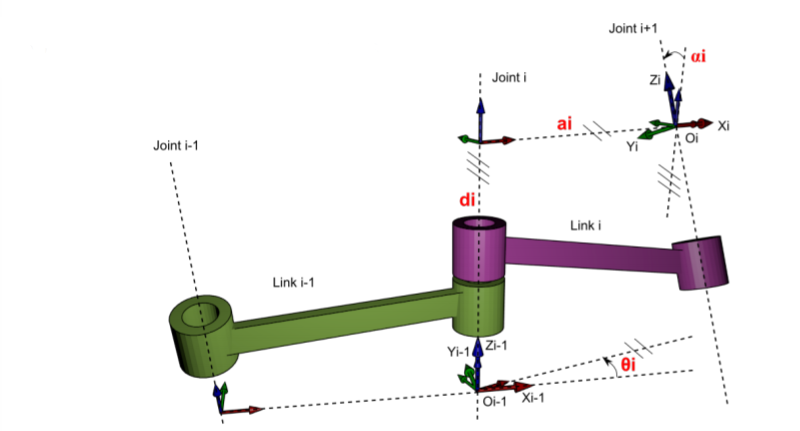
\includegraphics[width=0.45\linewidth]{images/dh.png}
    \caption{Robotic manipulator, with DH parametrization}
    \label{pict:dh}
\end{figure}

To compute forward kinematic problem, the Denavit-Hartenberg convention is usually used. This convention defines a transformation between frame {i} relative to the frame {i-1}. The general form of $T_i^{i-1}$:

\begin{equation}
    A_i = Rot_{z,\theta _i} Trans_{z,d_i} Trans_{x,a_i} Rot_{x, \alpha _i}
\end{equation}
with $A_i$, the transform between a link i and its parents i-1.
\begin{enumerate}
    \item z-axis of parent link i-1 aligned with axis of joint i
    \item 4 parameters for joint angle ($\theta _i$), link offset ($d_i$), link length ($a_i$), link twist ($\alpha _i$)
\end{enumerate}
Solving this transformation from base link to end effector link, the pose of the end effector can be compute what solves the forward kinematic problem. 

\subsection{Inverse kinematics}
\label{chap:inversekinematics}


Another method to control the pose of the end effector is the inverse method of the forward kinematic called inverse kinematic \cite{trove.nla.gov.au/work/27361264}. The inverse kinematics method calculates a set of all possible joints angles, which can be used to obtain desired position and orientation of the end effector. In terms of Denavit-Hartenberg convention, we are searching for an angle ($\theta _i$) with given $T_i^{i-1}$. In case of obtaining multiply solutions, decisions has to be taken to have an optimal motion in terms of various factors and constraints.
There is also possibility of nonexistence of the problem solution. It also might be state that point is not reachable for the manipulator. This method is subject to singularities, for example there are an infinite solution to reach the desired pose and the robot is lost on the one to choose. Local minima is another issue, the manipulator think that the pose has been reached but it is not, it is just a local minima. Finding the correct solution might be more complex than when using forward kinematics. They are a lot of different methods to solve inverse kinematic problems such as iterative methods or closed loop methods for example \cite{326569}.

The iterative methods solve the inverse kinematics problem by using a sequence of attempts leading to incrementally better configuration for the joints angles. Achieving better configuration means minimizing the difference between the current and target positions of the robot’s end-effector.

Another approach is closed-form method. In a closed-form method, the solution of the joints angles configuration can be straightforward expressed as a set of closed-form equations. Closed-form method gives a clear, single solution when is used for 6-degree-of-freedom systems with special kinematic structure
of kinematic chains

For mapping the joint velocities to the spatial velocities of the end effector expressed in word frame, the Jacobian matrix is used. For the work presented here, it is used given an end effector spatial velocity vector to compute the joint velocities to achieve this command as long as the Jacobian is non-singular.

\begin{equation}
    v_c = J(X) \Dot{\theta }
\end{equation}
with $v_c$, vector of spatial velocities and $\theta$, joint angles. 
\newpage